\begin{tcolorbox}[posterbox]
\SectionTitle{EEG Acquisition and Preprocessing}
\SmallText
\begin{itemize}
  \item 128-channel EGI Geodesic Sensor Net (250 Hz); online 0.1-100 Hz; offline low-pass 40 Hz.
  \item Epoch window: -100 to 600 ms relative to target onset.
  \item Components: P1, N1, P3b, and frontal MMN-like response at Fz.
  \item POT montage for P1/N1 and midline parietal montage for P3b.
\end{itemize}

\begin{center}
  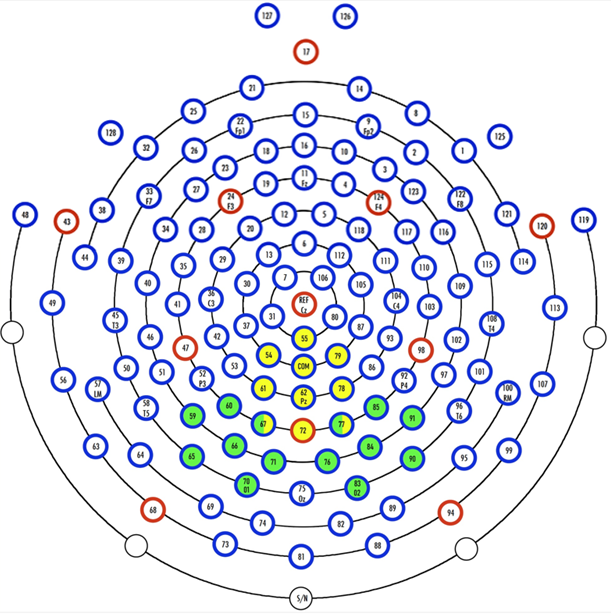
\includegraphics[width=0.70\linewidth]{media/electrodes.png}
\end{center}
\SmallText
\textbf{Fig. 2.} Electrode groupings used for averaging and analysis. Pz area shown in yellow and POT regions in green.
\end{tcolorbox}

\vspace{0.14in}

\begin{tcolorbox}[posterbox]
\SectionTitle{Behavioral Results: Distance and Direction}

\begin{center}
  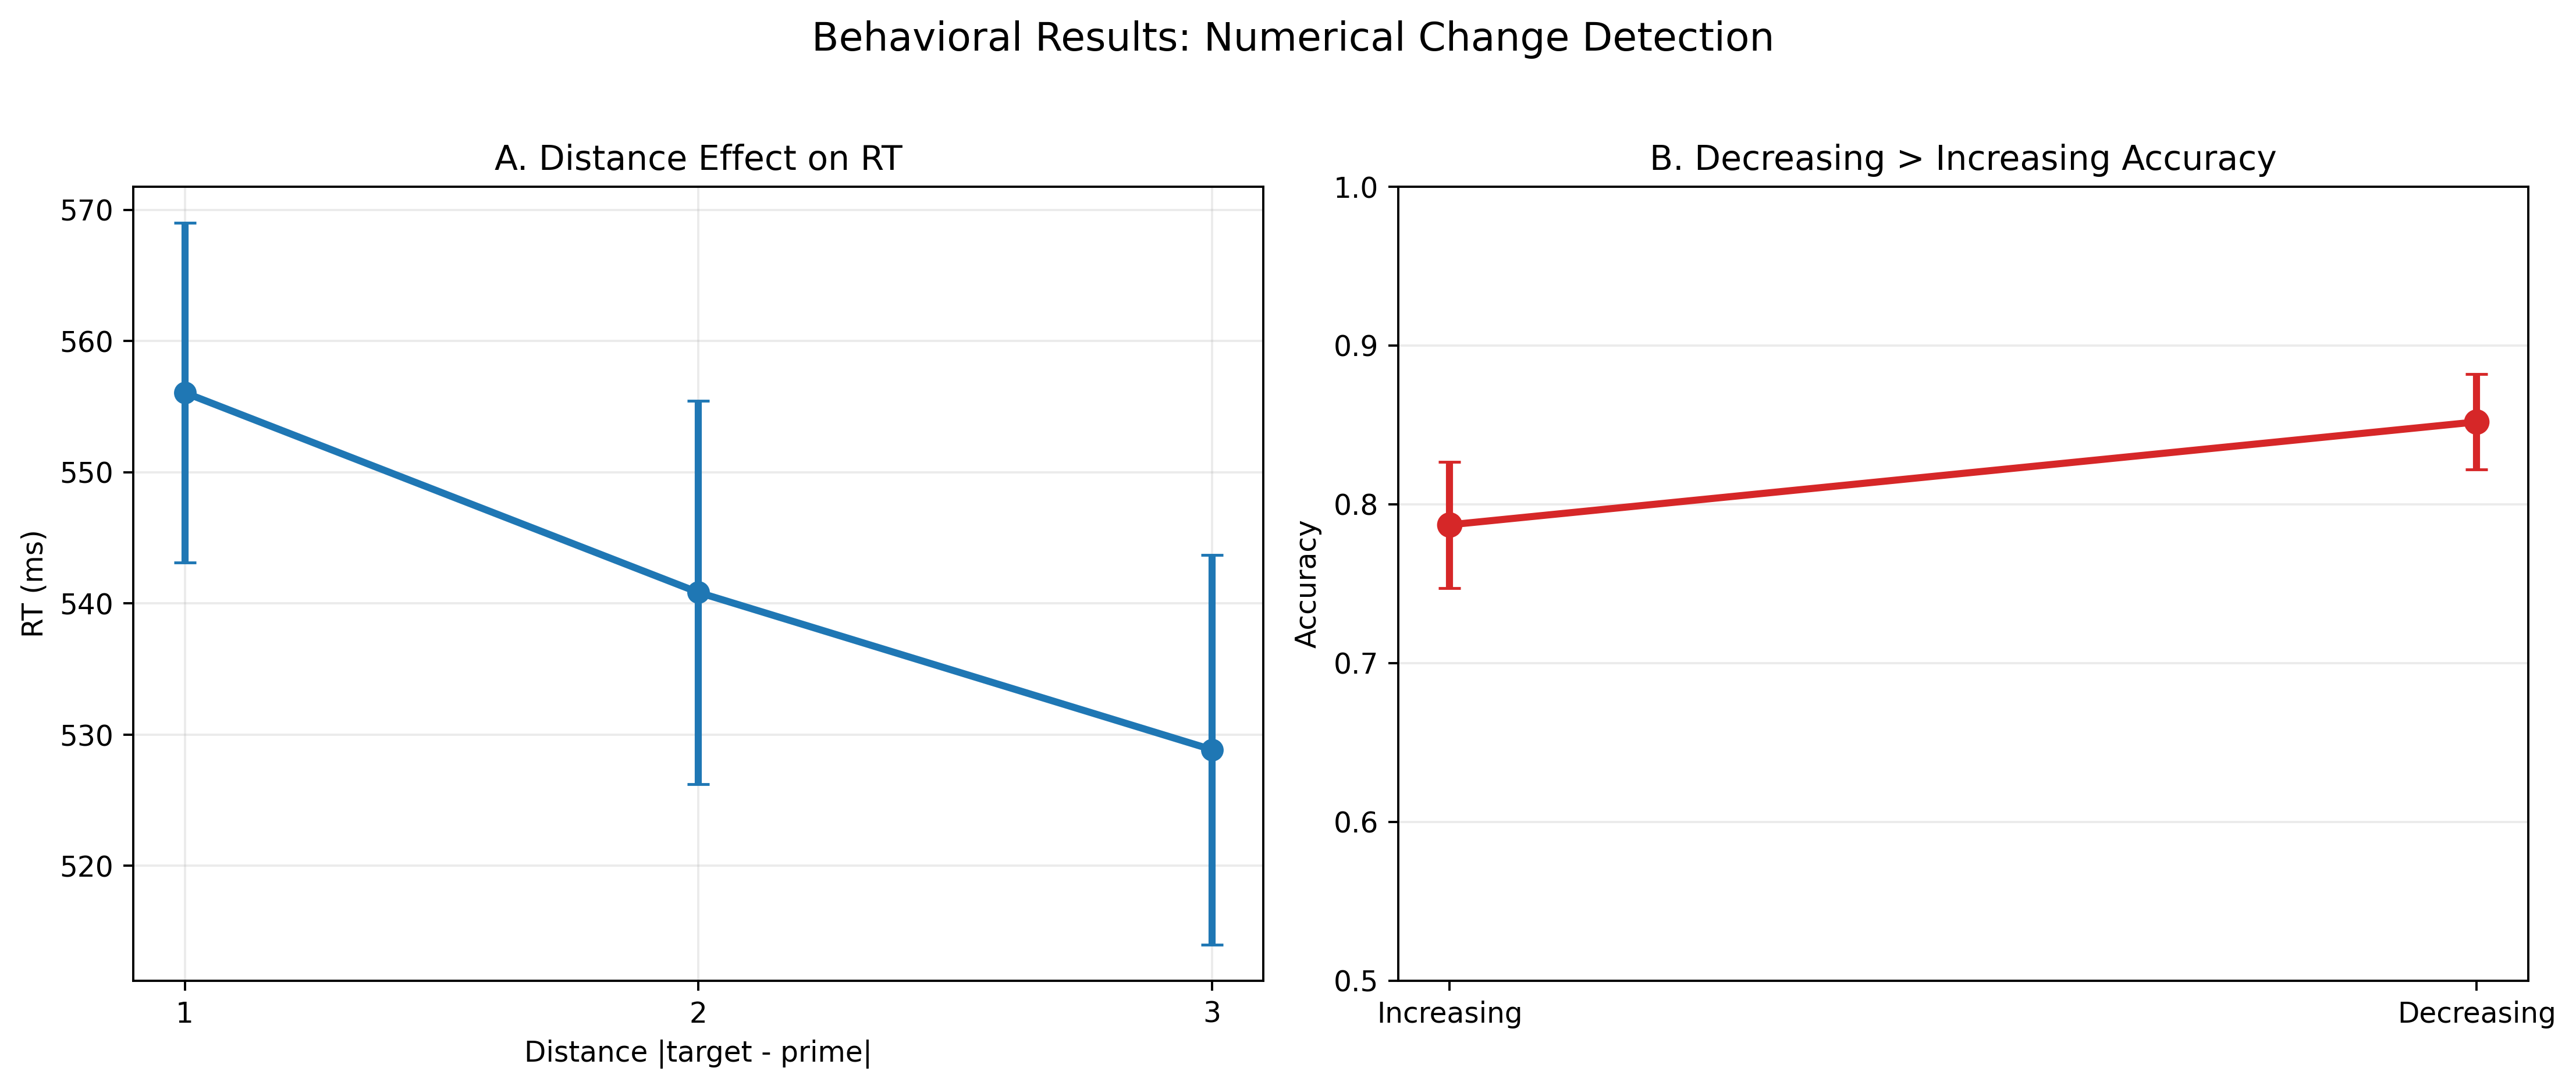
\includegraphics[width=0.92\linewidth]{../docs/assets/poster_plots/behavioral/behavior_poster_main.png}
\end{center}
\SmallText
\textbf{Fig. 3.} Left: RT decreases with larger numerical distance. Right: Decreasing changes are more accurate than Increasing changes.

\vspace{0.15em}
\textbf{Inference summary:}
\begin{itemize}
  \item \textbf{RT distance effect:} $b=-0.0261$, $SE=0.0033$, $p=5.31\times10^{-15}$ (about 2.57\% faster per distance step).
  \item \textbf{Accuracy direction effect:} OR(Decreasing vs Increasing) $=1.596$, 95\% CI [1.339, 1.904], $p=1.96\times10^{-7}$.
  \item \textbf{Subject-level confirmation (two-sided):} RT slope $=-13.60$ ms/step ($p=3.05\times10^{-7}$), accuracy D-I $=0.0648$ ($p=7.67\times10^{-5}$).
\end{itemize}
\end{tcolorbox}
